\PassOptionsToPackage{unicode=true}{hyperref} % options for packages loaded elsewhere
\PassOptionsToPackage{hyphens}{url}
%
\documentclass[]{article}
\usepackage{lmodern}
\usepackage{amssymb,amsmath}
\usepackage{ifxetex,ifluatex}
\usepackage{fixltx2e} % provides \textsubscript
\ifnum 0\ifxetex 1\fi\ifluatex 1\fi=0 % if pdftex
  \usepackage[T1]{fontenc}
  \usepackage[utf8]{inputenc}
  \usepackage{textcomp} % provides euro and other symbols
\else % if luatex or xelatex
  \usepackage{unicode-math}
  \defaultfontfeatures{Ligatures=TeX,Scale=MatchLowercase}
\fi
% use upquote if available, for straight quotes in verbatim environments
\IfFileExists{upquote.sty}{\usepackage{upquote}}{}
% use microtype if available
\IfFileExists{microtype.sty}{%
\usepackage[]{microtype}
\UseMicrotypeSet[protrusion]{basicmath} % disable protrusion for tt fonts
}{}
\IfFileExists{parskip.sty}{%
\usepackage{parskip}
}{% else
\setlength{\parindent}{0pt}
\setlength{\parskip}{6pt plus 2pt minus 1pt}
}
\usepackage{hyperref}
\hypersetup{
            pdftitle={Electrophysiological measures of visual suppression},
            pdfauthor={Daniel H. Baker \& Alex R. Wade},
            pdfborder={0 0 0},
            breaklinks=true}
\urlstyle{same}  % don't use monospace font for urls
\usepackage[margin=1in]{geometry}
\usepackage{longtable,booktabs}
% Fix footnotes in tables (requires footnote package)
\IfFileExists{footnote.sty}{\usepackage{footnote}\makesavenoteenv{longtable}}{}
\usepackage{graphicx,grffile}
\makeatletter
\def\maxwidth{\ifdim\Gin@nat@width>\linewidth\linewidth\else\Gin@nat@width\fi}
\def\maxheight{\ifdim\Gin@nat@height>\textheight\textheight\else\Gin@nat@height\fi}
\makeatother
% Scale images if necessary, so that they will not overflow the page
% margins by default, and it is still possible to overwrite the defaults
% using explicit options in \includegraphics[width, height, ...]{}
\setkeys{Gin}{width=\maxwidth,height=\maxheight,keepaspectratio}
\setlength{\emergencystretch}{3em}  % prevent overfull lines
\providecommand{\tightlist}{%
  \setlength{\itemsep}{0pt}\setlength{\parskip}{0pt}}
\setcounter{secnumdepth}{5}
% Redefines (sub)paragraphs to behave more like sections
\ifx\paragraph\undefined\else
\let\oldparagraph\paragraph
\renewcommand{\paragraph}[1]{\oldparagraph{#1}\mbox{}}
\fi
\ifx\subparagraph\undefined\else
\let\oldsubparagraph\subparagraph
\renewcommand{\subparagraph}[1]{\oldsubparagraph{#1}\mbox{}}
\fi

% set default figure placement to htbp
\makeatletter
\def\fps@figure{htbp}
\makeatother


\title{Electrophysiological measures of visual suppression}
\author{Daniel H. Baker \& Alex R. Wade}
\date{2021-02-26}

\begin{document}
\maketitle

\hypertarget{abstract}{%
\section{Abstract}\label{abstract}}

\hypertarget{introduction}{%
\section{Introduction}\label{introduction}}

Suppression is a fundamental component of the nervous system, and is critically important for moderating neural firing. Without suppression, neural activity would be too metabolically expensive, and uncontrolled excitation might lead to seizures. In the visual system, neurons responsive to a spatially localised narrowband target stimulus are suppressed by nearby neurons that differ in their tuning (Heeger, 1992). This tuning might involve different orientations (cross-orientation suppression), different spatial locations (lateral, or surround suppression), and different eye-of-origin (interocular suppression). Suppression is typically studied using a masking paradigm, where the response to a target stimulus is reduced by the presence of a high contrast mask (see examples in Figure \ref{fig:stimfig}a).

Several studies have demonstrated that these different types of suppression have distinct characteristics, and may occur at different stages in the early visual pathway. For example, suppression from an overlaid mask shown to the same eye as a target is immune to adaptation (Baker et al., 2007; Freeman et al., 2002), occurs at temporal frequencies above the range at which cortical neurons respond (Freeman et al., 2002; Li et al., 2005; Sengpiel and Vorobyov, 2005), and therefore appears consistent with a pre-cortical locus (Freeman et al., 2002; Li et al., 2005). If the mask is presented dichoptically (to the opposite eye from the target), suppression can be reduced by adaptation (Baker et al., 2007; Li et al., 2005; Sengpiel and Vorobyov, 2005), has a temporal profile consistent with cortical neurons (Li et al., 2005; Sengpiel and Vorobyov, 2005), and is reduced by applying bicuculline (a compound that blocks the suppressive neurotransmitter GABA) to early visual cortex (Sengpiel and Vorobyov, 2005). This points to a cortical locus for interocular suppression. Finally, surround masks have tighter tuning than overlaid masks, are most effective in the periphery (Petrov et al., 2005), and (in V1) cause suppression via feedback from higher visual areas (Nassi et al., 2013). Additionally, some studies have linked the magnitude of surround suppression with levels of GABA in early visual cortex (Cook et al., 2016; Yoon et al., 2010), again pointing to a cortical locus.

\begin{figure}

{\centering 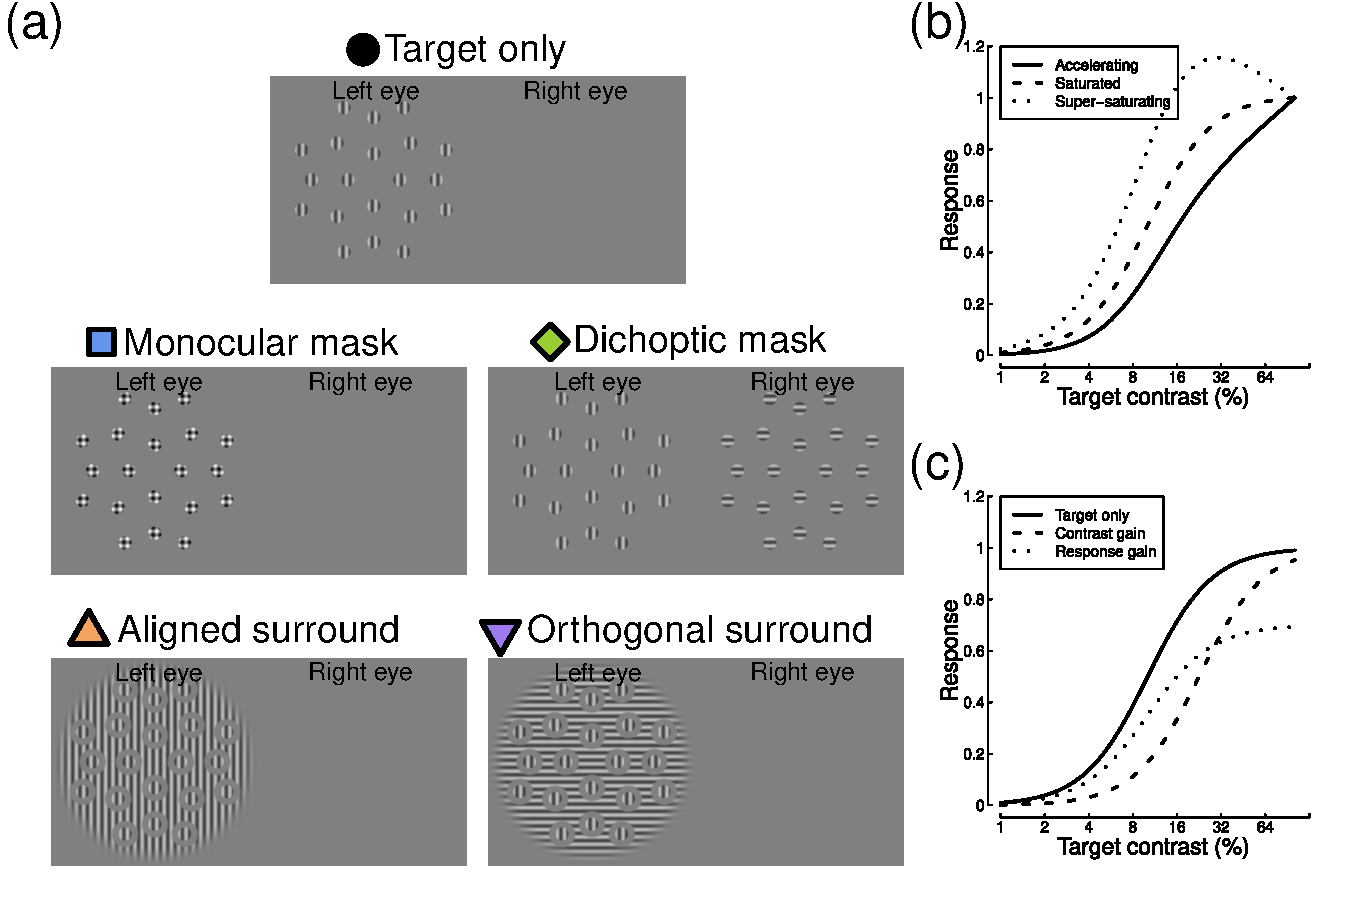
\includegraphics{figures/stimfig} 

}

\caption{Example stimuli and illustration of contrast response functions. Panel (a) shows four stimulus arrangments, illustrating how a vertical target pattern can be combined with four different mask types. Panel (b) shows three varieties of contrast response function, that either continue to accelerate (solid line), saturate (dashed line) or super-saturate (dotted line) across the range of displayable stimulus contrasts. Panel (c) illustrates a contrast gain (dashed line) and a response gain (dotted line) shift, relative to a baseline response (solid line).}\label{fig:stimfig}
\end{figure}

An important distinction concerns whether a suppressive effect modulates the contrast gain or the response gain of a neuron (or neural population). Changes in contrast gain shift the stimulus-response curve (the contrast response function) laterally, whereas changes in response gain scale the function vertically (see examples in Figure \ref{fig:stimfig}c). These different patterns may be indicative of specific neurophysiological underpinnings for an effect, and potentially different processes might occur at successive stages of processing. Previous studies have found that spatial attention modulates response gain (Itthipuripat et al., 2019), whereas suppression from overlaid masks is more consistent with contrast gain (Tsai et al., 2012). Spatial adaptation appears to affect both contrast and response gain in primary visual cortex (Albrecht et al., 1984), whereas motion adaptation is mostly attributable to contrast gain in area MT (Kohn and Movshon, 2003). In addition, there is evidence that suppression builds up at successive stages of cortical processing, beyond primary visual cortex, and is stronger at later levels in the visual hierarchy (Zenger-Landolt and Heeger, 2003). This is especially likely for surround suppression, which might be mediated by higher-level neurons with large receptive fields.

Neural responses can be measured non-invasively using steady-state visual evoked potentials (SSVEPs; Norcia et al., 2015) recorded with either electroencephalography (EEG) or magnetoencephalography (MEG). By flickering the target stimulus at a fixed frequency, entrained neural oscillations are evoked at the stimulus frequency, and also its higher harmonics (integer multiples of the flicker rate). Previous studies have shown that contrast-response functions measured using SSVEP are strongly modulated by overlaid masks (Baker and Vilidaitė, 2014; Busse et al., 2009; Tsai et al., 2012), dichoptic masks (Baker and Wade, 2017; Chadnova et al., 2018), and surround masks (Benjamin et al., 2018; Vanegas et al., 2015; Xiao and Wade, 2010). However the three types of mask have not been directly compared, and doing so is the main purpose of the present study. In particular, we were interested in determining whether each type of suppression is best described as a contrast gain or a response gain effect, and whether this changes across different electrode sites and different response frequencies. A secondary aim was to determine whether suppressive signals saturate as a function of contrast. We repeated our main experiment at two different mask contrasts, and analyse the data using a hierarchical Bayesian modelling approach.

\hypertarget{methods}{%
\section{Methods}\label{methods}}

\hypertarget{participants}{%
\subsection{Participants}\label{participants}}

Twelve participants completed each version of the experiment (3 participants completed both experiments, the remaining 9 were unique to each experiment). All participants had normal or corrected-to-normal vision, and no known visual abnormalities. Participants were briefed on the experimental protocols and purpose, and provided written informed consent.

\hypertarget{apparatus-and-stimuli}{%
\subsection{Apparatus and stimuli}\label{apparatus-and-stimuli}}

Stimuli were presented using a ViewPixx 3D display (VPixx Technologies Inc., Quebec, Canada), driven by a Mac Pro computer. The refresh rate was 120 Hz, and we interleaved frames intended for the left and right eyes (60 Hz refresh rate per eye). To enable stereo presentation, the display update was synchronised with a set of NVidia 3D pro active shutter glasses using an infra-red signal. The display had a resolution of 1920 \(\times\) 1280 pixels, and was viewed from a distance of 57cm, at which one degree of visual angle had a diameter of 36 pixels. To ensure good contrast resolution, the display was run in the high bit-depth monochrome M16 mode, which provided 16 bits of greyscale resolution. A Minolta LS110 photometer was used to gamma corrected the display, which had a maximum luminance of 102 \(cd/m^2\).

All stimuli were patches of sinusoidal grating with a spatial frequency of 1 cycle per degree. Target stimuli were randomly oriented on each trial, and windowed by a raised cosine envelope with a width of 2 degrees. There were 20 targets arranged in a symmetrical pattern around a central fixation marker, as shown in Figure \ref{fig:stimfig}a. The target eccentricities were 3.6, 7.1, 8.5 and 10.7 degrees from the central fixation. Stimuli were spaced in 90 degree intervals at each radius, or in 45 degree intervals at the largest eccentricity. All target stimuli flickered sinusoidally at 5Hz (on-off flicker), between 0\% contrast and their nominal Michelson contrast, which was one of six values (0, 6, 12, 24, 48 and 96\%). Percentage Michelson contrast is defined as \(100\frac{L_{max}-L_{min}}{L_{max}+L_{min}}\), where \emph{L} is luminance. Targets were shown to one eye only, which was chosen randomly on each trial. A binocular fixation marker was created from a cluster of overlaid squares (each 13 arc min wide) with random grey levels, designed to aid binocular fusion. Similar markers were also presented in the four corners of the stimulus region, at a distance of 15.7 degrees from the display centre.

We measured target responses with no mask, and also with four categories of mask stimulus. Monocular masks were shown to the same eye as the targets and in the same locations, but had orthogonal orientation. Dichoptic masks were the same, but shown to the non-target eye. Aligned surround masks were large (28 degrees in diameter) grating patches with the same orientation as the target, and with holes surrounding each target element (and the fixation marker). The holes were 4 degrees in diameter, meaning the gap between target and mask was 1 degree (one cycle of the stimulus waveform). Orthogonal surrounds were the same, but were oriented at 90 degrees relative to the targets. There were two principal mask contrasts that were used in the two versions of the experiment: 12\% and 24\%. We also tested several additional mask contrasts (6, 48 and 96\% contrast) for a single target contrast of 24\%. The masks drifted at a speed of 6 deg/sec so that the phase alignment between mask and target changed over time (Xiao and Wade, 2010). Note that drifting gratings do not produce a steady-state signal, so we did not record responses to the mask stimuli. In addition, for some of the monocular mask conditions, the target contrast was reduced from 96\% to 88\% or 68\% contrast to avoid clipping artifacts caused by overlaying the target and mask.

EEG activity was recorded using a 64-channel ANT Neuroscan system sampling at 1 kHz. Participants wore Waveguard caps, with electrodes organised according to the 10/20 system. The ground was located at position \emph{AFz}, and each channel was referenced to the whole-head average. Electrode impedance was maintained at or below 5 k\(\Omega\) throughout the experiment. Digital parallel triggers were sent from the ViewPixx display to the EEG amplifier, and recorded the onset of each trial on the EEG trace. Data were amplified, digitised, and saved to disc for offline analysis.

\hypertarget{procedure}{%
\subsection{Procedure}\label{procedure}}

After providing consent, participants were set up with an EEG cap of appropriate size. They then completed six blocks, each comprising a full repetition of the experiment. Blocks lasted around 10 minutes, with the opportunity to take breaks between blocks. Within each block, all 42 conditions were repeated once in a randomized order. Trials lasted 11 seconds, with an inter-trial interval of 3 seconds. Participants were asked to monitor the central fixation and, as far as possible, to minimise blinking when a stimulus was displayed. To maintain attention, the central fixation marker was changed occasionally by resampling the positions and luminances of the squares. There was a 50\% chance of this happening on each trial. Participants were asked to count the number of times the fixation marker changed, and report this at the end of the block.

\hypertarget{data-analysis-and-modelling}{%
\subsection{Data analysis and modelling}\label{data-analysis-and-modelling}}

All data were converted from the native ANT-EEProbe format to a compressed comma-separated value (csv) text file using a custom \emph{Matlab} script and components of the EEGlab toolbox (Delorme and Makeig, 2004). The data for each participant were then loaded into \emph{R} for analysis. A ten-second waveform for each trial at each electrode was extracted, omitting the first one second after stimulus onset to avoid transients. The fast Fourier transform was calculated for each waveform, and the spectrum stored in a matrix. All repetitions of each condition were then coherently averaged (i.e.~taking both the phase and amplitude into account), before being converted to a signal-to-noise ratio by dividing the amplitude at each frequency by the mean amplitude of the neighbouring 10 bins (\(\pm0.5\) Hz in steps of 0.1 Hz). The signal-to-noise ratio at the target flicker frequency (5 Hz) and its second harmonic (10 Hz) were then used as dependent variables for further analysis.

Our primary objective was to understand the relative contributions of contrast gain and response gain to suppression from different mask types. We quantified this using a two-stage hierarchical Bayesian modelling approach, which incorporates the data from individual participants. At the first stage, we fitted a gain control model with three free parameters to the baseline data. The model is defined as:

\begin{equation}
\label{eq:GC1}
resp = R_{max}\frac{C^p}{Z + C^2} + 1,
\end{equation}

where \emph{C} is the target contrast. The \(Z\) parameter sets the horizontal position, \(p\) governs the function shape from accelerating (\emph{p} \textgreater{} 2) to saturating (\emph{p} = 2) to super-saturating (\emph{p} \textless{} 2), and \(R_{max}\) scales the overall height of the function. The additive constant (+1) represents additive noise, and converts the response to a signal-to-noise ratio (implicitly, we also divide \emph{resp} by 1, but this is omitted as it has no effect). We fitted the model to each participant's baseline data, and obtained estimates of the three free parameters independently at each electrode location. The hyperpriors for each parameter were normal distributions with parameters: \(\mu\) = 50, \(\sigma\) = 20 (\emph{Z}); \(\mu\) = 2, \(\sigma\) = 0.25 (\emph{p}); and \(\mu\) = 4, \(\sigma\) = 2 (\(R_{max}\)). All parameters were constrained to have positive values.

The second stage of fitting used the mean posterior parameter estimates from the first stage (for each participant), and fitted the contrast response function for each mask type using the equation:

\begin{equation}
\label{eq:GC2}
resp = \frac{R_{max}}{r} \times \frac{C^p}{gZ + C^2} + 1,
\end{equation}

where the new terms \emph{r} and \emph{g} are free parameters that govern the extent of response gain and contrast gain, respectively. Values of \emph{r}, \emph{g} \textgreater{} 1 indicate suppression, though in principle masks can also cause facilitation (\emph{r}, \emph{g} \textless{} 1). We estimated values of these parameters jointly at each electrode location and for each mask type, again using the data from all participants in a hierarchical model. We defined broad hyperpriors for \emph{g} and \emph{r} as gamma distributions, with parameters \(\alpha\) = 1.5, \(\beta\) = 0.5 {[}MAYBE CHANGE TO 1.2 AND 0.2{]}. These functions peak at \(\frac{\alpha-1}{\beta}\) = 1, so the prior expectation before observing empirical data is that there is no suppression of either kind. The priors had greater probability mass at values \textgreater{} 1, reflecting our expectation that one or both parameters would produce suppression, but also extended below 1, ensuring that the model was also capable of capturing facilitation where it appeared in the data. Bayesian modelling was implemented in \emph{Stan} (Carpenter et al., 2017), based on an example script for hierarchical nonlinear regression accompanying Chapter 17 of Kruschke (2014). We examined how the posterior mean of each parameter varied as a function of mask type, electrode position, and response frequency.

\hypertarget{data-and-script-availability}{%
\subsection{Data and script availability}\label{data-and-script-availability}}

All data and scripts are publicly available at: \url{https://osf.io/e62wu/}

\hypertarget{results}{%
\section{Results}\label{results}}

The target stimulus evoked strong steady-state responses at both the first harmonic frequency (5 Hz) and the second harmonic frequency (10 Hz). Figure \ref{fig:fftfig}a shows the averaged Fourier spectrum from the baseline (no mask) condition with 96\% target contrast. Responses at both frequencies were strongest at the occipital pole, over early visual cortex (see inset scalp plots). At most electrodes, responses increased monotonically as a function of contrast (see examples in Figure \ref{fig:fftfig}b,c). In general, responses at the first harmonic (5Hz) were more likely to accelerate, and those at the second harmonic more likely to saturate or super-saturate. The scalp plot insets to Figures \ref{fig:fftfig}b,c summarise this using a saturation index proposed by Ledgeway et al. (2005). It was calculated by taking the difference between the responses at the highest two contrasts (96\% and 48\%), and dividing by the maximum response. Values of SI \textgreater{} 1 correspond to acceleration (plotted violet), SI = 1 to saturation (white), and SI \textless{} 1 to super-saturation (green). Notice that overall the first harmonic responses accelerate (median SI = 0.10), but that many of the second harmonic responses saturate or super-saturate (median SI = 0.01).

\begin{figure}

{\centering 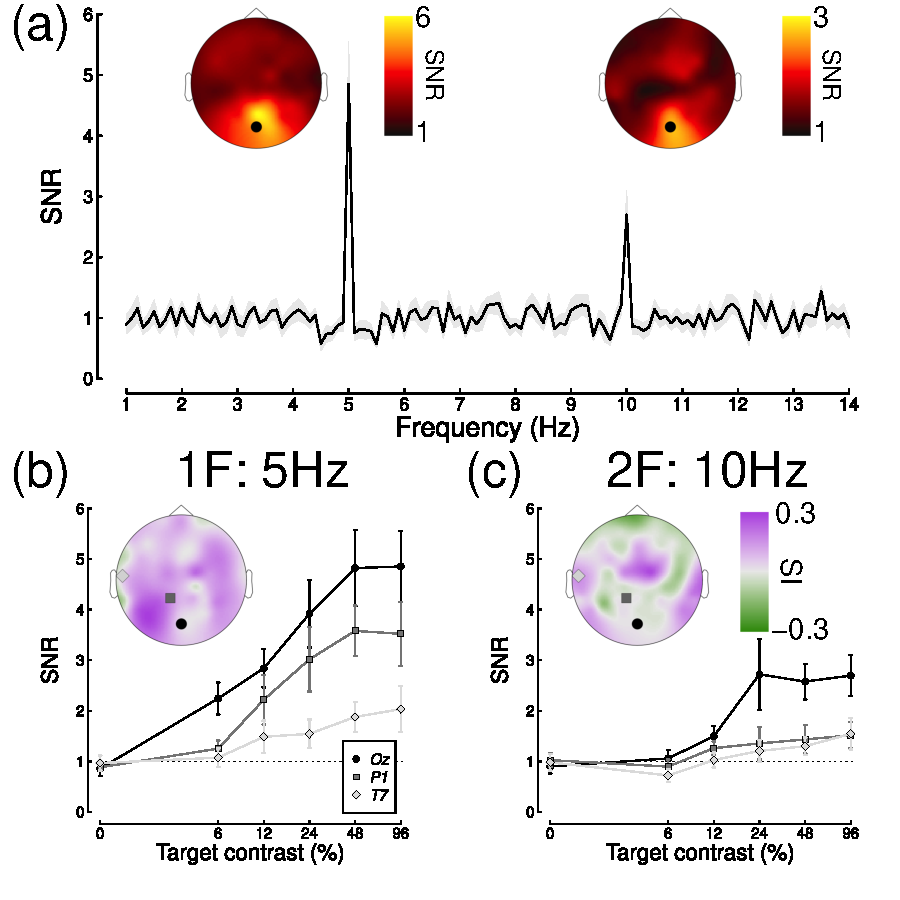
\includegraphics{figures/fftfig} 

}

\caption{Averaged Fourier spectrum and example contrast response functions. Panel (a) shows the spectrum for a high contrast target, with inset scalp plots showing SNRs at the first and second harmonic frequencies. The spectrum is taken from electrode Oz, indicated by the black points in the scalp plots. The shaded region and error bars indicate ±1 standard error. Panels (b) and (c) show example contrast response functions at the first and second harmonics at electrodes Oz, P1 and T7, averaged across participants (N=12). The inset scalp plots show how the saturation index varies across the head.}\label{fig:fftfig}
\end{figure}

To quantify how suppression varied across the scalp, and across different mask types and response frequencies, we fitted a hierarchical Bayesian model to the data. The first stage of this process involved estimating values for the free parameters in equation \eqref{eq:GC1}. Figure \ref{fig:modelfig1}a shows an example fit at electrode \emph{Oz} for the low contrast mask experiment. The thick black line gives the fit using the posterior mean parameter estimates (\emph{p} = 1.94, \emph{Z} = 134.35, \(R_{max}\) = 4.8), and thin lines show predictions for 100 randomly sampled posterior parameter combinations. At the second stage of fitting, we estimated values of the suppressive parameters \emph{g} and \emph{r} for each mask type. Example fits are shown in Figure \ref{fig:modelfig1}b-e, with accompanying posterior distributions of parameter estimates in panels g-j. We assess whether a parameter makes a credible contribution to the response by determining whether the 95\% highest density interval of the posterior (shown by the black bars at the margins of Figure \ref{fig:modelfig1}g-j) encompasses 1. For all four examples shown in Figure \ref{fig:modelfig1}g-j, the contrast gain parameter (\emph{g}, y-axis) was credibly greater than 1, whereas the response gain parameter (\emph{r}, x-axis) was not credibly different from 1. This is evidence that all four mask types modulate responses via contrast gain control at electrode \emph{Oz}, for the first harmonic response.

\begin{figure}

{\centering 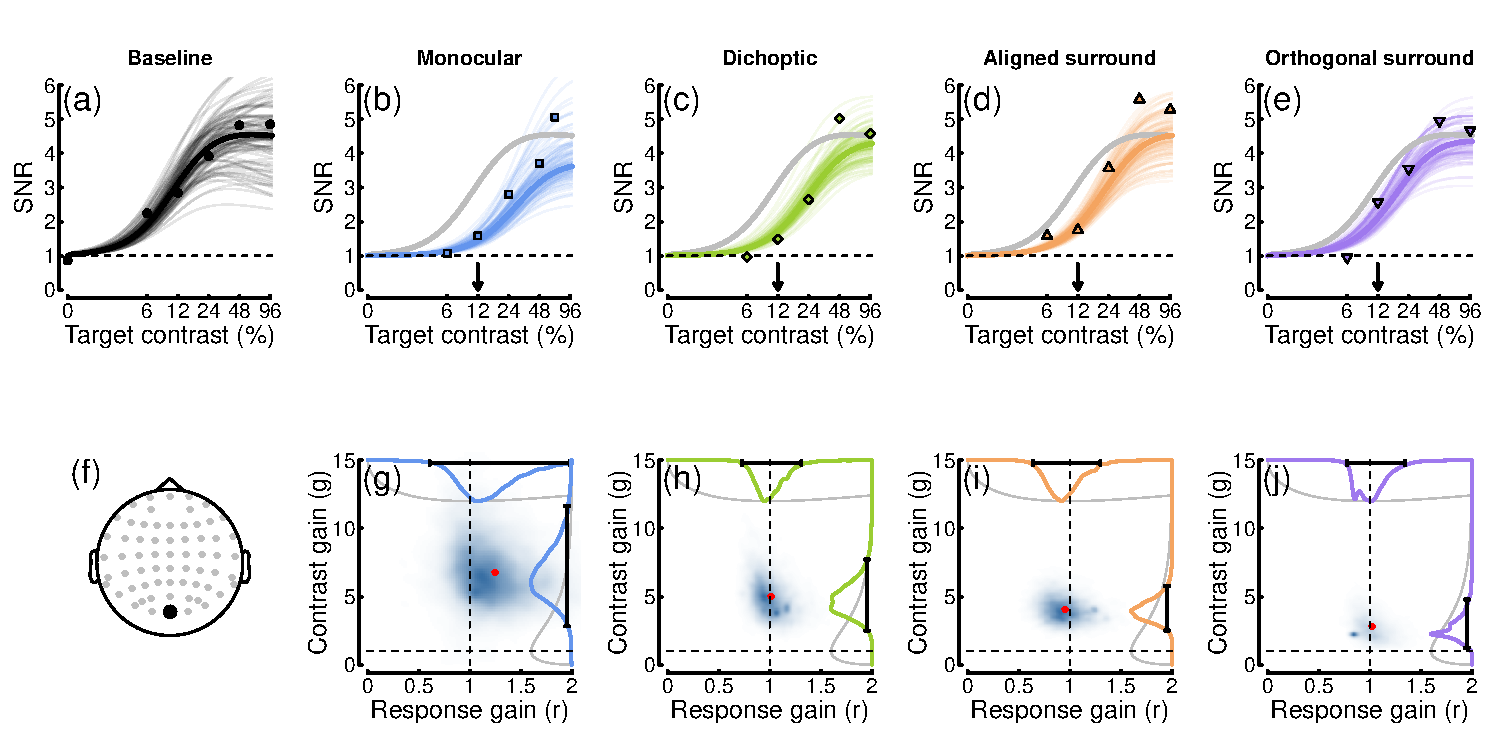
\includegraphics{figures/modelfig1} 

}

\caption{Contrast response functions from electrode Oz, with example model fits and posterior parameter estimates. Panel (a) shows the data from the baseline (no mask) condition (points), plotted alongside model curves for the posterior mean of parameter estimates (thick curve), and random posterior samples (thin curves). Panels (b-e) show data for four types of masks in the same format (grey curves duplicate the mean fit from panel (a)), with the arrows indicating the mask contrast. Panel (f) shows the electrode location. Panels (g-j) show posterior density estimates for the response gain (x-axis) and contrast gain (y-axis) weight parameters. Red points show the means, dashed lines give the value expected in the case of no effect (a weight of 1), and grey and coloured distributions in the margins show the prior and posterior for each parameter. For all mask types, the contrast gain weight estimate was substantially greater than 1.}\label{fig:modelfig1}
\end{figure}

We repeated the above analysis independently at each electrode, for each response frequency (5 Hz and 10 Hz), and for both experiments (12\% and 24\% mask contrast). Figure \ref{fig:modelheads1} summarises the results for the 12\% mask contrast experiment, and for each mask type. For the first harmonic (5 Hz) response (top two rows), there were strong contrast gain control effects (panels a-d), but little credible effect of response gain (panels e-h). For the second harmonic response (10 Hz), although some contrast gain effects were credible at the occipital pole (electrode \emph{Oz} for all mask types, panels i-l), suppression was better described by response gain (panels m-p). Example contrast response functions and posterior distributions at the second harmonic are shown in Figure \ref{fig:modelfig2}. This overall pattern was replicated in our second data set with higher (24\%) contrast masks (Figure \ref{fig:modelheads2}).

\begin{figure}

{\centering 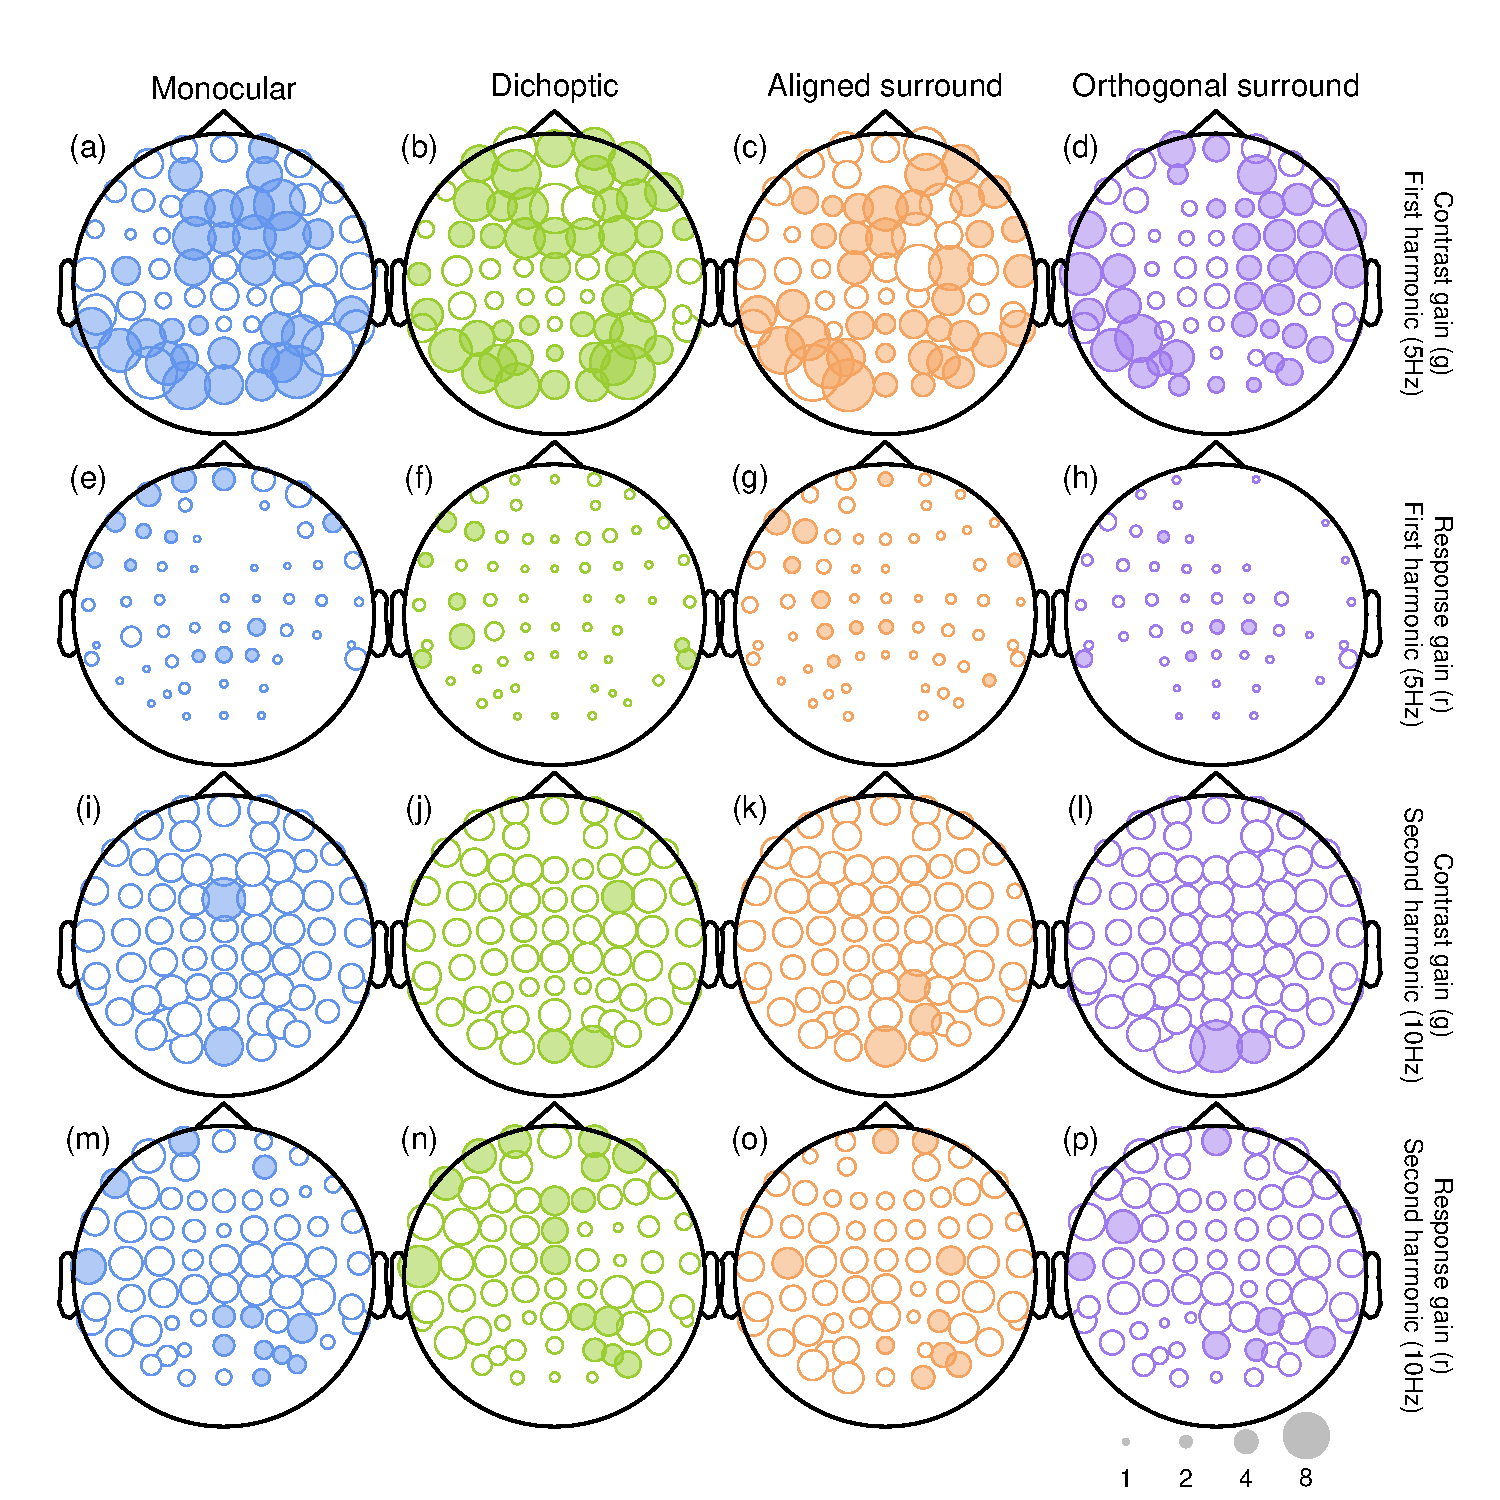
\includegraphics{figures/modelheads1} 

}

\caption{Scalp plots summarising the suppressive weights for contrast and response gain from the Bayesian hierarchical model, fitted to data from the low mask contrast experiment. Symbols are filled white when the 95 percent highest density interval of the posterior parameter distribution includes 1 (implying no credible contribution from that type of suppression). Larger symbols correspond to stronger suppression (see the scale in lower right corner), but parameters implying facilitation (values < 1) are not plotted.}\label{fig:modelheads1}
\end{figure}

\begin{figure}

{\centering 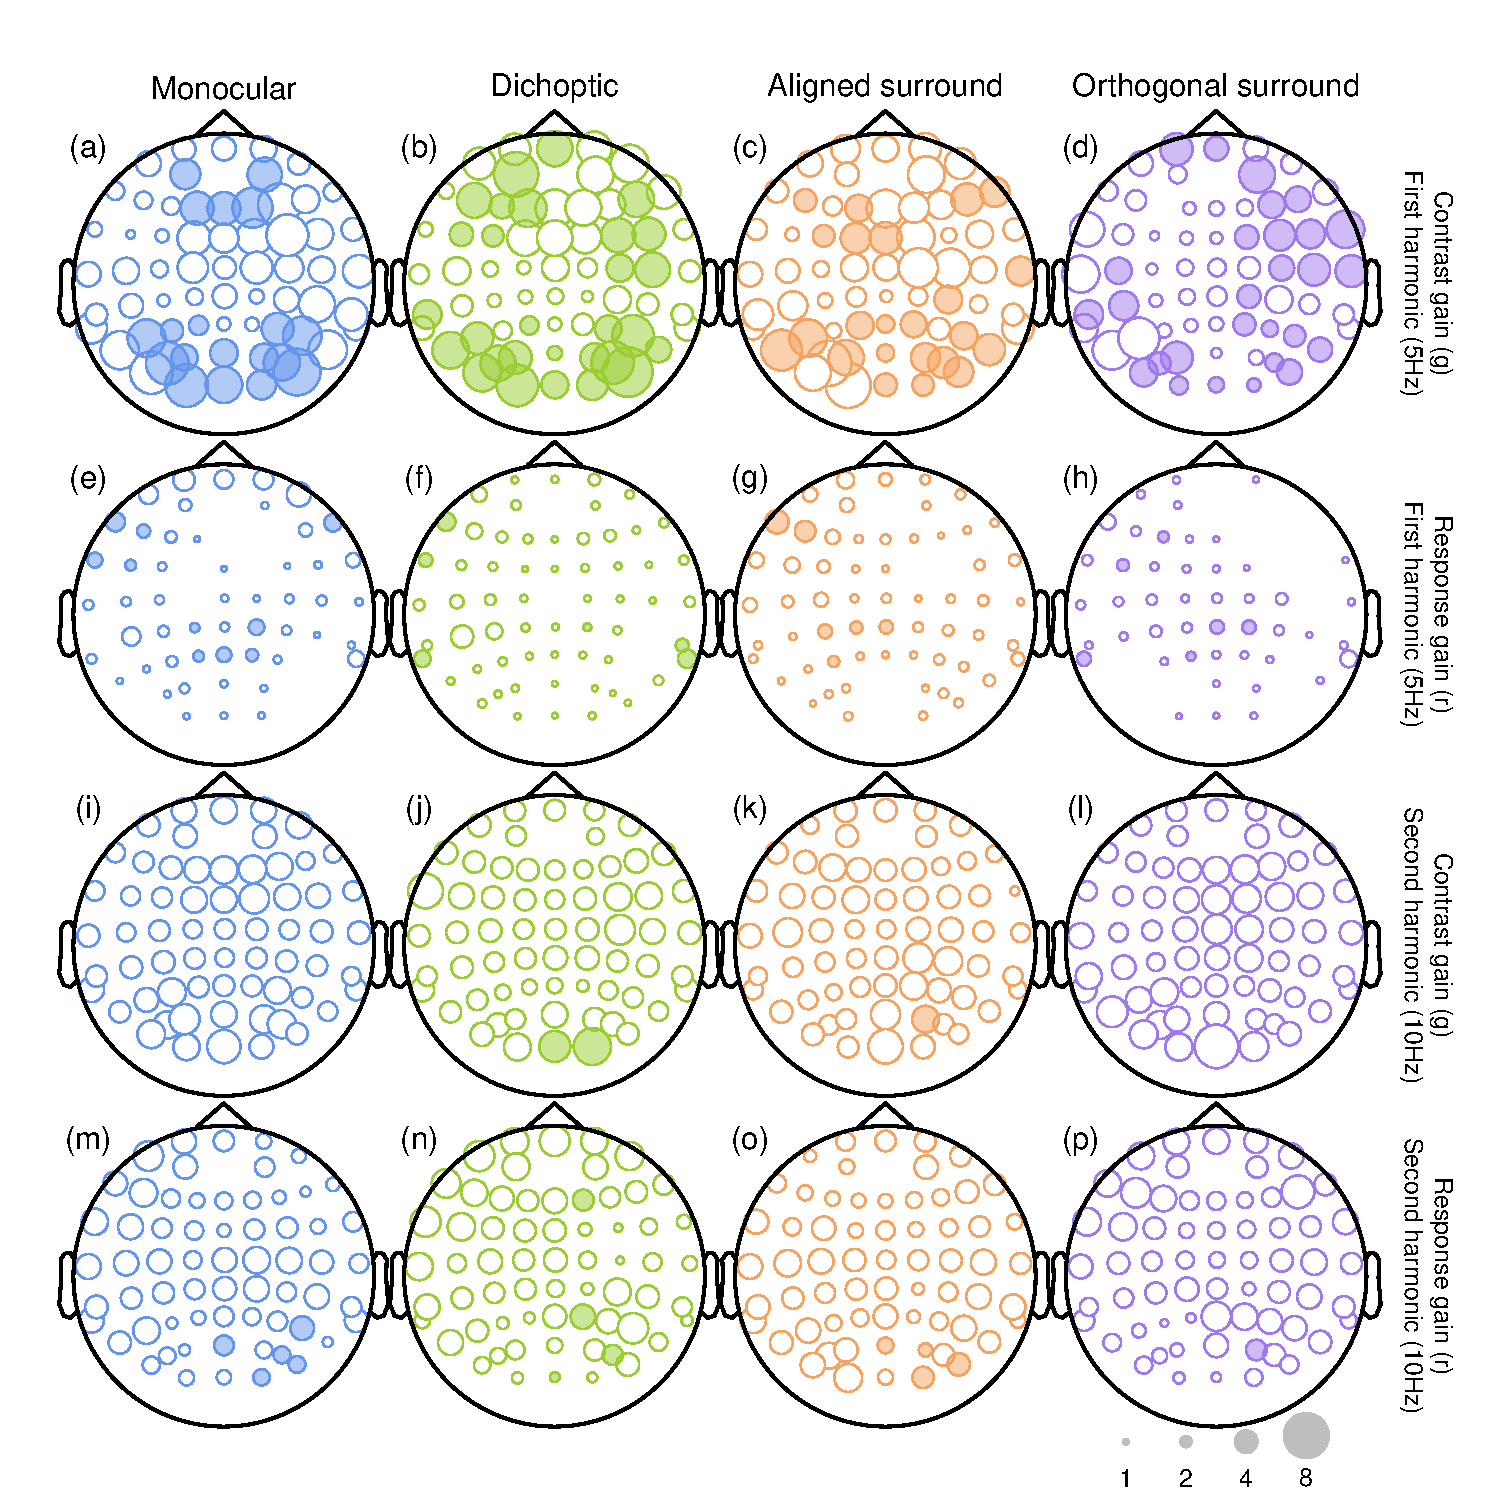
\includegraphics{figures/modelfig2} 

}

\caption{Contrast response functions at the second harmonic frequency. Plotting conventions mirror those in Figure 3. Note that the lower SNR at 10 Hz results in noisier data and less precise posterior estimates than at 5 Hz.}\label{fig:modelfig2}
\end{figure}

Closer inspection of these results reveals some interesting subtleties and differences across mask conditions. Note in particular that the weights for surround suppression at the first harmonic are generally weaker at the occipital pole (electrodes \emph{Oz} and \emph{POz}) than for monocular and dichoptic suppression. But suppressive weights increase at more lateral electrodes over more parietal regions of cortex. For surround suppression, this might reflect the increased suppression in extra-striate cortical regions that have larger receptive fields. More generally, it also suggests that suppression builds up across successive stages of processing. It also appears that, whereas suppression at the first harmonic is primarily due to contrast gain control, suppression at the second harmonic involves changes in both contrast and response gain (see lower two rows of Figures \ref{fig:modelheads1} \& \ref{fig:modelheads2}). This may well reflect the involvement of different classes of neurons - for example, second harmonic responses imply more severe nonlinearities, which might include suppression. This is also consistent with the greater saturation of the second harmonic response (inset to Figure \ref{fig:modelfig1}c).

\begin{figure}

{\centering 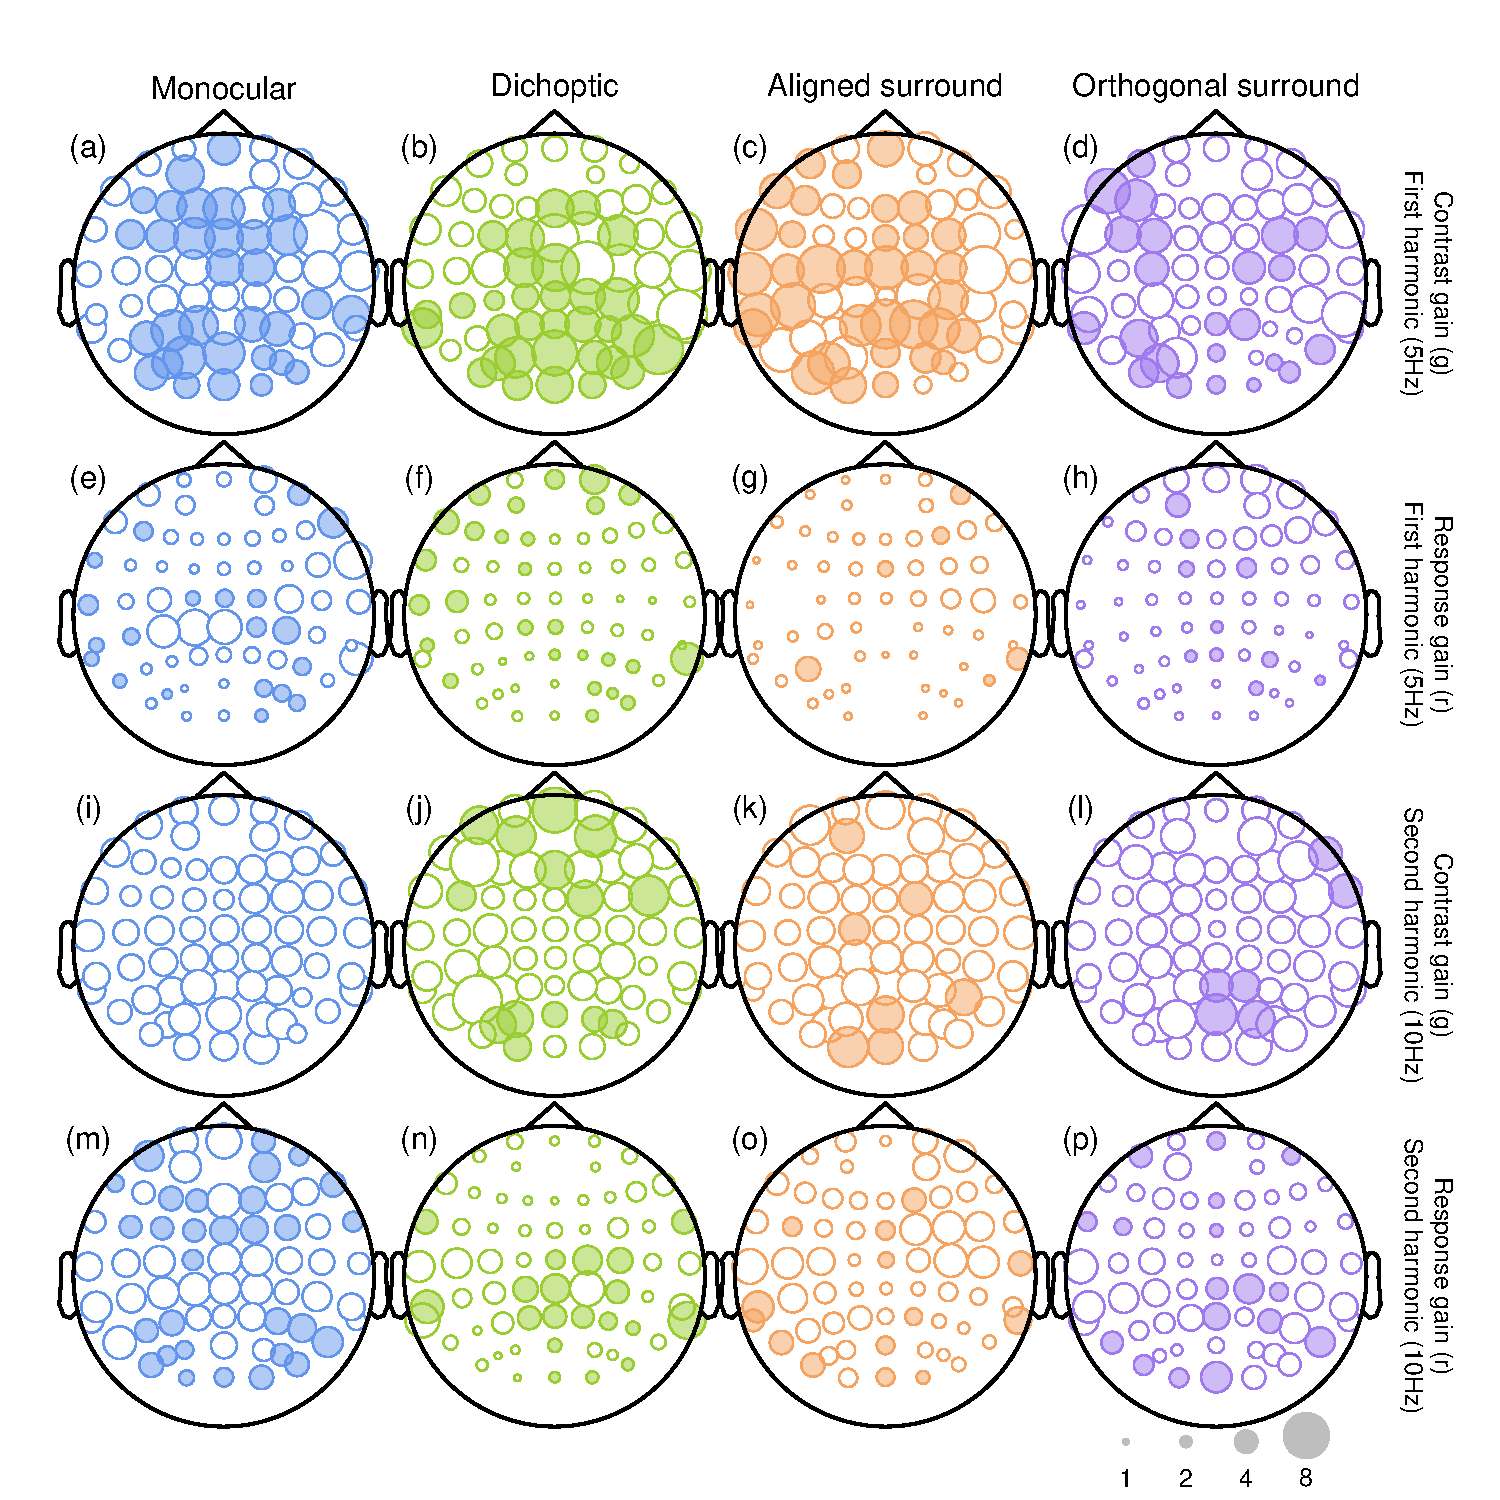
\includegraphics{figures/modelheads2} 

}

\caption{Scalp plots summarising the suppressive weights for contrast and response gain from the Bayesian hierarchical model, fitted to data from the high mask contrast experiment. Plotting conventions are as for Figure 4.}\label{fig:modelheads2}
\end{figure}

Finally, we asked about the properties of the mask signal. Of particular interest is whether the mask signal itself saturates before suppressing the target. If it does, this implies the presence of a nonlinearity before suppression impacts, as has been shown psychophysically for surround masks (Meese et al., 2009). Figure \ref{fig:masksignals}a shows model predictions for a linear suppressive signal (black curve), and a saturating suppressive signal (blue curve).

We also measured responses at a fixed target contrast (24\%), for mask contrasts that ranged from 0\% to 96\%. For this analysis, we pooled data across the two experiments, giving us N = 21 participants (data for the three participants who completed both experiments were averaged to give a single data set for each of those participants). The results for all four mask types are shown in Figure \ref{fig:masksignals}b-e.

\begin{figure}

{\centering 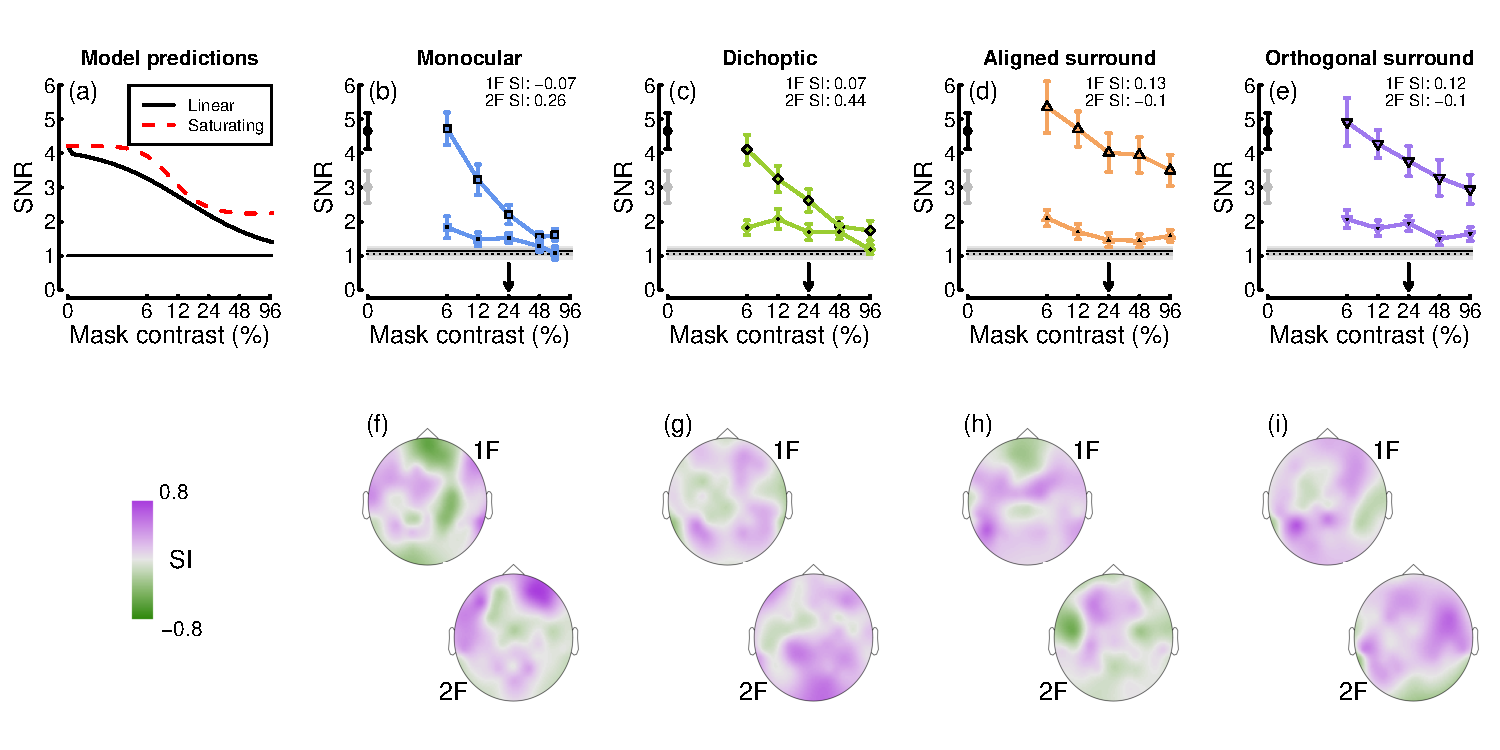
\includegraphics{figures/masksignals} 

}

\caption{.}\label{fig:masksignals}
\end{figure}

\hypertarget{discussion}{%
\section{Discussion}\label{discussion}}

We asked whether suppression from four types of mask could be best explained by changes in contrast gain or response gain. Data from two SSVEP experiments showed that at the first harmonic frequency, all four mask types were best explained by contrast gain control, with minimal influence from response gain. However at the second harmonic frequency, both types of gain control were apparent. There was also evidence that the strength of suppression, particularly from the surround, increased away from the occipital pole. Finally, we showed that the suppressive signals from surround masks saturate before impacting the target, suggesting they have passed through a nonlinearity before suppressing other signals.

\hypertarget{distinct-suppressive-pathways-with-a-common-outcome}{%
\subsection{Distinct suppressive pathways with a common outcome}\label{distinct-suppressive-pathways-with-a-common-outcome}}

\hypertarget{are-previous-ssvep-studies-also-consistent-with-contrast-gain-effects}{%
\subsection{Are previous SSVEP studies also consistent with contrast gain effects?}\label{are-previous-ssvep-studies-also-consistent-with-contrast-gain-effects}}

(The plan here is to repeat the same Bayesian modelling on data from the literature. Here are 16 studies that report data for one of the mask types. Please add more if you can think of them.)

\emph{Overlay}

Baker \& Vilidaite 2014

Smith 2017

Tsai 2012

Busse 2009 Fig 6c

Candy 2001

Ross \& Speed 1991

Burr \& Morrone 1987

\emph{Dichoptic}

Chadnova 2018

Baker \& Wade 2017

Baker 2015

Zhou 2015

Hou 2020

\emph{Surround}

Vanegas 2015

Benjamin 2018

Ohtani 2002 Fig 7

Vanegas 2019

Figure 8: summary of meta-analysis

What about the Mannion data? We could potentially ask to include it, and add him as an author.

\hypertarget{what-is-suppression-for}{%
\subsection{What is suppression for?}\label{what-is-suppression-for}}

Mention normalization reweighting and optimal combination

\hypertarget{acknowledgements}{%
\section{Acknowledgements}\label{acknowledgements}}

Supported by the Royal Society (grant number RG130121 to DHB).

\hypertarget{references}{%
\section*{References}\label{references}}
\addcontentsline{toc}{section}{References}

\hypertarget{refs}{}
\leavevmode\hypertarget{ref-Albrecht1984}{}%
Albrecht DG, Farrar SB, Hamilton DB. 1984. Spatial contrast adaptation characteristics of neurones recorded in the cat's visual cortex. \emph{J Physiol} \textbf{347}:713--39. doi:\href{https://doi.org/10.1113/jphysiol.1984.sp015092}{10.1113/jphysiol.1984.sp015092}

\leavevmode\hypertarget{ref-Baker2007}{}%
Baker DH, Meese TS, Summers RJ. 2007. Psychophysical evidence for two routes to suppression before binocular summation of signals in human vision. \emph{Neuroscience} \textbf{146}:435--48. doi:\href{https://doi.org/10.1016/j.neuroscience.2007.01.030}{10.1016/j.neuroscience.2007.01.030}

\leavevmode\hypertarget{ref-Baker2014}{}%
Baker DH, Vilidaitė G. 2014. Broadband noise masks suppress neural responses to narrowband stimuli. \emph{Front Psychol} \textbf{5}:763. doi:\href{https://doi.org/10.3389/fpsyg.2014.00763}{10.3389/fpsyg.2014.00763}

\leavevmode\hypertarget{ref-Baker2017}{}%
Baker DH, Wade AR. 2017. Evidence for an optimal algorithm underlying signal combination in human visual cortex. \emph{Cereb Cortex} \textbf{27}:254--264. doi:\href{https://doi.org/10.1093/cercor/bhw395}{10.1093/cercor/bhw395}

\leavevmode\hypertarget{ref-Benjamin2018}{}%
Benjamin AV, Wailes-Newson K, Ma-Wyatt A, Baker DH, Wade AR. 2018. The effect of locomotion on early visual contrast processing in humans. \emph{J Neurosci} \textbf{38}:3050--3059. doi:\href{https://doi.org/10.1523/JNEUROSCI.1428-17.2017}{10.1523/JNEUROSCI.1428-17.2017}

\leavevmode\hypertarget{ref-Busse2009}{}%
Busse L, Wade AR, Carandini M. 2009. Representation of concurrent stimuli by population activity in visual cortex. \emph{Neuron} \textbf{64}:931--42. doi:\href{https://doi.org/10.1016/j.neuron.2009.11.004}{10.1016/j.neuron.2009.11.004}

\leavevmode\hypertarget{ref-Carpenter2017}{}%
Carpenter B, Gelman A, Hoffman MD, Lee D, Goodrich B, Betancourt M, Brubaker M, Guo J, Li P, Riddell A. 2017. Stan: A probabilistic programming language. \emph{Journal of Statistical Software, Articles} \textbf{76}:1--32. doi:\href{https://doi.org/10.18637/jss.v076.i01}{10.18637/jss.v076.i01}

\leavevmode\hypertarget{ref-Chadnova2018}{}%
Chadnova E, Reynaud A, Clavagnier S, Baker DH, Baillet S, Hess RF. 2018. Interocular interaction of contrast and luminance signals in human primary visual cortex. \emph{Neuroimage} \textbf{167}:23--30. doi:\href{https://doi.org/10.1016/j.neuroimage.2017.10.035}{10.1016/j.neuroimage.2017.10.035}

\leavevmode\hypertarget{ref-Cook2016}{}%
Cook E, Hammett ST, Larsson J. 2016. GABA predicts visual intelligence. \emph{Neurosci Lett} \textbf{632}:50--4. doi:\href{https://doi.org/10.1016/j.neulet.2016.07.053}{10.1016/j.neulet.2016.07.053}

\leavevmode\hypertarget{ref-Delorme2004}{}%
Delorme A, Makeig S. 2004. EEGLAB: An open source toolbox for analysis of single-trial eeg dynamics including independent component analysis. \emph{J Neurosci Methods} \textbf{134}:9--21. doi:\href{https://doi.org/10.1016/j.jneumeth.2003.10.009}{10.1016/j.jneumeth.2003.10.009}

\leavevmode\hypertarget{ref-Freeman2002}{}%
Freeman TCB, Durand S, Kiper DC, Carandini M. 2002. Suppression without inhibition in visual cortex. \emph{Neuron} \textbf{35}:759--71. doi:\href{https://doi.org/10.1016/s0896-6273(02)00819-x}{10.1016/s0896-6273(02)00819-x}

\leavevmode\hypertarget{ref-Heeger1992}{}%
Heeger DJ. 1992. Normalization of cell responses in cat striate cortex. \emph{Vis Neurosci} \textbf{9}:181--97. doi:\href{https://doi.org/10.1017/s0952523800009640}{10.1017/s0952523800009640}

\leavevmode\hypertarget{ref-Itthipuripat2019}{}%
Itthipuripat S, Sprague TC, Serences JT. 2019. Functional mri and eeg index complementary attentional modulations. \emph{J Neurosci} \textbf{39}:6162--6179. doi:\href{https://doi.org/10.1523/JNEUROSCI.2519-18.2019}{10.1523/JNEUROSCI.2519-18.2019}

\leavevmode\hypertarget{ref-Kohn2003}{}%
Kohn A, Movshon JA. 2003. Neuronal adaptation to visual motion in area mt of the macaque. \emph{Neuron} \textbf{39}:681--91. doi:\href{https://doi.org/10.1016/s0896-6273(03)00438-0}{10.1016/s0896-6273(03)00438-0}

\leavevmode\hypertarget{ref-Kruschke2014}{}%
Kruschke JK. 2014. Doing Bayesian data analysis: a tutorial with R, JAGS, and Stan, 2nd ed. Elsevier, Academic Press.

\leavevmode\hypertarget{ref-Ledgeway2005}{}%
Ledgeway T, Zhan C, Johnson AP, Song Y, Baker CL Jr. 2005. The direction-selective contrast response of area 18 neurons is different for first- and second-order motion. \emph{Vis Neurosci} \textbf{22}:87--99. doi:\href{https://doi.org/10.1017/S0952523805221120}{10.1017/S0952523805221120}

\leavevmode\hypertarget{ref-Li2005}{}%
Li B, Peterson MR, Thompson JK, Duong T, Freeman RD. 2005. Cross-orientation suppression: Monoptic and dichoptic mechanisms are different. \emph{J Neurophysiol} \textbf{94}:1645--50. doi:\href{https://doi.org/10.1152/jn.00203.2005}{10.1152/jn.00203.2005}

\leavevmode\hypertarget{ref-Meese2009}{}%
Meese TS, Challinor KL, Summers RJ, Baker DH. 2009. Suppression pathways saturate with contrast for parallel surrounds but not for superimposed cross-oriented masks. \emph{Vision Res} \textbf{49}:2927--35. doi:\href{https://doi.org/10.1016/j.visres.2009.09.006}{10.1016/j.visres.2009.09.006}

\leavevmode\hypertarget{ref-Nassi2013}{}%
Nassi JJ, Lomber SG, Born RT. 2013. Corticocortical feedback contributes to surround suppression in v1 of the alert primate. \emph{J Neurosci} \textbf{33}:8504--17. doi:\href{https://doi.org/10.1523/JNEUROSCI.5124-12.2013}{10.1523/JNEUROSCI.5124-12.2013}

\leavevmode\hypertarget{ref-Norcia2015}{}%
Norcia AM, Appelbaum LG, Ales JM, Cottereau BR, Rossion B. 2015. The steady-state visual evoked potential in vision research: A review. \emph{J Vis} \textbf{15}:4. doi:\href{https://doi.org/10.1167/15.6.4}{10.1167/15.6.4}

\leavevmode\hypertarget{ref-Petrov2005}{}%
Petrov Y, Carandini M, McKee S. 2005. Two distinct mechanisms of suppression in human vision. \emph{J Neurosci} \textbf{25}:8704--7. doi:\href{https://doi.org/10.1523/JNEUROSCI.2871-05.2005}{10.1523/JNEUROSCI.2871-05.2005}

\leavevmode\hypertarget{ref-Sengpiel2005}{}%
Sengpiel F, Vorobyov V. 2005. Intracortical origins of interocular suppression in the visual cortex. \emph{J Neurosci} \textbf{25}:6394--400. doi:\href{https://doi.org/10.1523/JNEUROSCI.0862-05.2005}{10.1523/JNEUROSCI.0862-05.2005}

\leavevmode\hypertarget{ref-Tsai2012}{}%
Tsai JJ, Wade AR, Norcia AM. 2012. Dynamics of normalization underlying masking in human visual cortex. \emph{J Neurosci} \textbf{32}:2783--9. doi:\href{https://doi.org/10.1523/JNEUROSCI.4485-11.2012}{10.1523/JNEUROSCI.4485-11.2012}

\leavevmode\hypertarget{ref-Vanegas2015}{}%
Vanegas MI, Blangero A, Kelly SP. 2015. Electrophysiological indices of surround suppression in humans. \emph{J Neurophysiol} \textbf{113}:1100--9. doi:\href{https://doi.org/10.1152/jn.00774.2014}{10.1152/jn.00774.2014}

\leavevmode\hypertarget{ref-Xiao2010}{}%
Xiao B, Wade AR. 2010. Measurements of long-range suppression in human opponent s-cone and achromatic luminance channels. \emph{J Vis} \textbf{10}:10. doi:\href{https://doi.org/10.1167/10.13.10}{10.1167/10.13.10}

\leavevmode\hypertarget{ref-Yoon2010}{}%
Yoon JH, Maddock RJ, Rokem A, Silver MA, Minzenberg MJ, Ragland JD, Carter CS. 2010. GABA concentration is reduced in visual cortex in schizophrenia and correlates with orientation-specific surround suppression. \emph{J Neurosci} \textbf{30}:3777--81. doi:\href{https://doi.org/10.1523/JNEUROSCI.6158-09.2010}{10.1523/JNEUROSCI.6158-09.2010}

\leavevmode\hypertarget{ref-Zenger-Landolt2003}{}%
Zenger-Landolt B, Heeger DJ. 2003. Response suppression in v1 agrees with psychophysics of surround masking. \emph{J Neurosci} \textbf{23}:6884--93.

\end{document}
